\pdfmapfile{+FSMe.map}
\documentclass[ProofPDF]{./Styles/Jnls-Template-V3}

\usepackage{booktabs}
\makeatletter
\gdef\printartdetails{\corresfont\par\ignorespaces\textbf{\color{BlueTextColor}STATUS:}\par\addvspace{-2pt}Manuscript in preparation for TISMIR. Not yet peer reviewed.}
\makeatother
\rectoheadtop{TAKA KHOO\ \ {\color{75black}\textit{Manuscript in preparation for TISMIR}}}
\versoheadtop{TAKA KHOO\ \ {\color{75black}\textit{Manuscript in preparation for TISMIR}}}

\begin{document}

\jname{Transactions of the International Society for Music Information Retrieval }
\jvol{00}
\jissue{00}
\jmonth{season}
\jyear{xxx}
\jid{doi}
\artid{xx.xxxx/xxxx.xx}
\filename{main}
\def\MSFirstPage{\pageref{startPage_Label}}
\def\MSLastPage{\pageref{endPage_Label}}
\graphicspath{{./figures/}}
\label{startPage_Label}
\title{Transposed Twins: Benchmark Leakage and Memorization in Symbolic Melody Models}

\articletype{RESEARCH ARTICLE}

\author[1]{Taka Khoo}
\howtociteauthor[1]{Taka Khoo}
\rhauthor[1]{T. Khoo}

\aff[1]{Independent researcher, \href{mailto:takakhoo@gmail.com}{takakhoo@gmail.com}}
\afflnote{*Author affiliations can be found in the back matter of this article}

\begin{history}
\submitted{\submittedday{xxx}\submittedmonth{xxx}\submittedyear{xxx}}
\accepted{\acceptedday{xxx}\acceptedmonth{xxx}\acceptedyear{xxx}}
\published{\publishedday{xxx}\publishedmonth{xxx}\publishedyear{xxx}}
\end{history}

\begin{abstract}[ABSTRACT]
Symbolic melody models are compared by how well they predict held-out melodies, but folk tunes, hymn tunes and popular songs circulate in many versions, often in different keys. We build a transposition- and tempo-invariant near-duplicate detector (interval and rhythm-ratio shingles, MinHash candidates, exact verification; recall 0.99 against exhaustive search) and audit eight melody corpora and their standard splits. In the JSB Chorales benchmark, 36\% of the official test chorales carry a soprano that shares at least half its phrases with a training chorale, and 13\% are transposed copies; a polyphonic fingerprint finds none, because Bach harmonized the same hymn tunes more than once. A random split of PDMX would give half of all test melodies a twin in training, and 6.2\% of PDMX's own deduplicated subset still has a transposed copy inside it. Retraining every model with and without the 25 training chorales that twin a test chorale prices the leak: 0.55 nats per note for a 4-gram model and 0.01 to 0.06 for transformers, rising with size. On the official test set the 4-gram beats every transformer we train (2.28 against 2.37 nats per note); on the clean test chorales the larger transformers win (2.51 against 2.83). On PDMX, models up to 7.4M parameters reproduce neither inserted canaries nor training melodies, and transposition augmentation is what suppresses memorization. A leak can thus inflate a benchmark with no detectable memorization. We release the detector, twin lists, leakage-free splits and a listening page.
\end{abstract}

\begin{keyword}[KEYWORDS:]
Symbolic music, melody, benchmark leakage, near-duplicate detection, memorization, evaluation, open data
\end{keyword}

\maketitle

\linenumbers

%%%%%%%%%%%%%%%%%%%%%%%%%%%%%%%%%%%%%%%%%%%%%%%%%%%%%%%%%%%%%%%%%%%%%%%%%%%%%%%%
\section{Introduction}\label{sec:intro}

Likelihood on held-out pieces is the standard yardstick for symbolic music models. Since \cite{boulangerlewandowski2012} released piano-roll splits of the JSB Chorales, Nottingham, MuseData and Piano-midi.de collections, papers on recurrent, convolutional and attention models have reported their negative log-likelihood on the same test sets \citep{huang2017coconet,bai2018tcn,huang2019musictransformer}, and melody corpora such as Essen \citep{schaffrath1995essen}, Hooktheory \citep{donahue2022sheetsage}, POP909 \citep{wang2020pop909} and PDMX \citep{long2025pdmx} feed the newer generation of melody and lead-sheet models. A held-out likelihood measures generalization only if the held-out pieces are new to the model.

Melodies make that condition easy to break. A hymn tune is harmonized many times; a folk tune is collected in many villages; a popular song is transcribed by many users. The versions differ in key, in tempo notation, and in a few ornaments, so file hashes and metadata matching miss them. In text and images, near-duplicates between training and test data inflate reported scores \citep{lee2022dedup,barz2020cifar,allamanis2019duplication,magar2022contamination}, and the music community has found duplicates inside the Lakh MIDI dataset \citep{choi2025lmddedup}. We found no audit of the standard melody splits with a detector that ignores transposition, and no measurement of what such leaks do to the numbers that papers report.

This article does both. Our contributions are:

\begin{enumerate}
\item A transposition- and tempo-invariant twin detector for melodies, with exact verification of every candidate and measured recall (Section~\ref{sec:method}).
\item An audit of eight corpora and their standard or customary splits (Section~\ref{sec:audit}). The JSB Chorales test set is 36\% leaked at the melody level and 0\% at the polyphonic level. PDMX is half near-duplicates.
\item A causal estimate of what the leak is worth, from retraining with and without the twins (Section~\ref{sec:counterfactual}). Copy-prone models gain an order of magnitude more than transformers, enough to reverse a model ranking, and among transformers the gain grows with size.
\item A controlled memorization study on PDMX with inserted canaries, natural duplicate families and a strict free-sample copy search (Section~\ref{sec:memorization}). Models at this scale do not reproduce training melodies; transposition augmentation is what keeps them from it.
\item Released resources: the detector, twin lists for every corpus we may redistribute, leakage-free splits, and an interactive page where the twins can be heard (Section~\ref{sec:release}).
\end{enumerate}

%%%%%%%%%%%%%%%%%%%%%%%%%%%%%%%%%%%%%%%%%%%%%%%%%%%%%%%%%%%%%%%%%%%%%%%%%%%%%%%%
\section{Related work}\label{sec:related}

\paragraph{Contamination in machine learning benchmarks.} \cite{lee2022dedup} found that over 4\% of validation examples in standard language-model corpora have a near-duplicate in training, and that perplexity on those examples is about half that on the rest. \cite{barz2020cifar} found near-duplicates of CIFAR test images in the training set and showed that removing them changes model rankings slightly. \cite{recht2019imagenet} rebuilt the ImageNet test set and saw accuracy drop across all models. In code, duplicated files inflate metrics for models of source code \citep{allamanis2019duplication}. For large language models, contamination is now measured per benchmark \citep{magar2022contamination,sainz2023contamination}. Our study transfers these questions to melody, where the natural notion of a duplicate is invariant to key and tempo and a byte-level or token-level match is too strict.

\paragraph{Duplicates in music corpora.} \cite{choi2025lmddedup} estimate that at least 21\% of the Lakh MIDI dataset is near-duplicated and argue that random splits skew cross-entropy, leaving the measurement of that effect to future work. PDMX removes duplicate scores using metadata and note counts \citep{long2025pdmx}. \cite{walder2016beyond} builds splits that keep transcriptions of the same piece together for a MIDI archive and keeps the original JSB split. \cite{leemhuis2019bacher} note that a chorale melody can appear in both training and test data because Bach harmonized hymn tunes repeatedly, without quantifying it. \cite{fathi2026howfarback} show that random splits of folk-tune renderings put another rendering of the same tune in training for most test sequences, then regroup by token patterns that are not transposition-invariant. Melodic similarity and plagiarism detection is a long-standing MIR task \citep{yin2021goodalgorithm,yin2022originality,lu2025melodysim}; we borrow its invariances and use them for data auditing.

\paragraph{Memorization.} Language models emit verbatim training text, and extraction grows with duplication and model size \citep{carlini2021extracting,carlini2023quantifying}; deduplicating training data reduces it \citep{kandpal2022dedupprivacy,lee2022dedup}. Audio generators replicate training clips \citep{bralios2024replication,batlleroca2024replication}. Music transformers lose transposition equivariance as they scale, which \cite{guo2026emt} read as capacity spent on absolute patterns. For symbolic melody models we found no measurement of verbatim extraction. Evaluation critiques argue that deep music models gain less over simple Markov baselines than reported \citep{yin2023shallowgains}; our counterfactual shows one mechanism by which a benchmark can favour the copy-prone baseline.

%%%%%%%%%%%%%%%%%%%%%%%%%%%%%%%%%%%%%%%%%%%%%%%%%%%%%%%%%%%%%%%%%%%%%%%%%%%%%%%%
\section{Finding transposed twins}\label{sec:method}

\subsection{Representation}
A melody is a sequence of notes with MIDI pitch $p_i$, onset $t_i$ and duration $d_i$ in quarter-note beats; rests are dropped and folded into the following inter-onset interval. Each note after the second is mapped to a symbol
\begin{align}\label{eq:symbol}
s_i = \Big(\operatorname{clip}(p_i - p_{i-1}, \pm 24),\; q\big(\tfrac{t_i - t_{i-1}}{t_{i-1} - t_{i-2}}\big)\Big),
\end{align}
the pitch interval to the previous note and a quantized ratio of successive inter-onset intervals. The ratio quantizer $q$ has nine bins with edges at $0.26, 0.41, 0.59, 0.84, 1.19, 1.68, 2.38$ and $3.36$, roughly geometric around 1. The symbols are unchanged by transposition and by uniform tempo scaling, so a tune written in quarter notes and the same tune in eighth notes map to the same string. For the piano-roll benchmarks, where only frames are available, the top voice is read as frame-to-frame pitch differences with markers for silence.

\subsection{Candidate search and verification}
Each melody becomes the set of hashed $k$-grams of its symbol string with $k=8$. MinHash \citep{broder1997resemblance} with 128 permutations, banded into 32 bands of four rows \citep{indyk1998ann}, proposes candidate pairs. Every candidate whose shingle Jaccard similarity is at least 0.15 is then verified exactly, with two scores: the Jaccard similarity $J$ of the shingle sets, which tolerates local edits and ornaments, and the longest common contiguous run of symbols. We call two melodies \textit{twins} if $J \geq 0.5$ or they share a run of at least 12 consecutive symbols, and a \textit{transposed copy} if $J \geq 0.9$. Families are connected components of the twin graph. On the JSB sopranos and on Nottingham, where every pair can be compared exhaustively, the candidate stage recovers 98.6\% and 100\% of the pairs with $J \geq 0.5$ and all pairs with $J \geq 0.9$. For the JSB benchmark tables we skip the candidate stage and compare every test piece with every training piece.

The thresholds are deliberately conservative. A pair at $J = 0.5$ shares half of its eight-note phrases in order-free terms, which in the folk and chorale data we inspected almost always means the same tune with variants. Melodies shorter than 16 symbols are excluded because short strings collide by chance.

%%%%%%%%%%%%%%%%%%%%%%%%%%%%%%%%%%%%%%%%%%%%%%%%%%%%%%%%%%%%%%%%%%%%%%%%%%%%%%%%
\section{An audit of eight corpora}\label{sec:audit}

\subsection{Corpora}
We audit the four piano-roll benchmarks of \cite{boulangerlewandowski2012} in the distribution used by \cite{bai2018tcn}, reading the top voice of each piece (the chorales were first assembled for machine learning by \citealt{allan2005harmonising}), and four melody corpora: the Essen folksong collection \citep{schaffrath1995essen} (8,382 melodies), the Nottingham database in its cleaned release \citep{jukedeck2017nottingham} (1,033 tunes), the melody tracks of POP909 \citep{wang2020pop909} (909 songs), the Hooktheory release of \cite{donahue2022sheetsage} (21,881 melody segments), and PDMX \citep{long2025pdmx}, from which we take the 220,902 public-domain or CC0 scores without licence conflicts and read a melody as the highest sounding note at each onset. All counts are after dropping melodies shorter than 16 symbols. The Session and IrishMAN are left out because The Session's content licence forbids processing its tunes with language-model tools \citep{thesession2026data}.

For corpora with an official split we report the fraction of test melodies with a twin in the training split. For corpora usually split at random, we draw 200 random 80/10/10 splits and report the mean fraction of test melodies with a twin in training, together with the 5th and 95th percentiles.

\subsection{Results}

% ------------------------------------------------------------
\begin{table*}[t]
\centering
\small
\begin{tabular}{llrrrrrl}
\toprule
\colhead{Corpus} & \colhead{Split} & \colhead{Melodies} & \colhead{With twin} & \colhead{With copy} & \colhead{Families} & \colhead{Largest} & \colhead{Test with twin in train} \\
\midrule
JSB Chorales (soprano) & official & 381 & 42.3\% & 17.6\% & 47 & 10 & \textbf{36.4\%} (copy 13.0\%) \\
 & random & & & & & & 38.5\% [26.7, 51.4] \\
PDMX & random & 220,902 & 53.8\% & 39.2\% & 34,945 & 89 & \textbf{49.7\%} [49.1, 50.2] \\
\quad PDMX dedup subset & & 75,915 & 15.2\% & 6.2\% & & & \\
Essen & random & 8,382 & 16.1\% & 8.4\% & 632 & 6 & 13.2\% [11.5, 14.9] \\
Nottingham & official & 1,033 & 5.3\% & 1.5\% & 27 & 3 & 2.4\% \\
 & random & & & & & & 4.4\% [1.9, 8.2] \\
MuseData (top voice) & official & 124 test & & & & & 2.4\% \\
Piano-midi.de (top voice) & official & 25 test & & & & & 0\% \\
Hooktheory & official (by artist) & 21,881 & 3.5\% & 1.7\% & 347 & 18 & 0.7\% (copy 0.35\%) \\
 & random & & & & & & 2.8\% [2.4, 3.4] \\
POP909 & random & 909 & 0.4\% & 0.2\% & 2 & 2 & 0.3\% [0.0, 1.2] \\
\bottomrule
\end{tabular}
\caption{Transposed twins in eight melody corpora. \textit{With twin} and \textit{with copy}: share of all melodies that have at least one twin ($J \geq 0.5$ or a 12-symbol common run) or transposed copy ($J \geq 0.9$) anywhere in the corpus. \textit{Test with twin in train}: share of test melodies with a twin in the training split; for random splits, the mean over 200 random 80/10/10 splits with the 5th and 95th percentiles in brackets. The PDMX dedup subset row counts twins inside the subset that PDMX itself marks as deduplicated. Nottingham's official row is the split of \cite{boulangerlewandowski2012}.}
\label{tab:audit}
\end{table*}
% ------------------------------------------------------------

% ------------------------------------------------------------
\begin{figure*}[t]
\centering
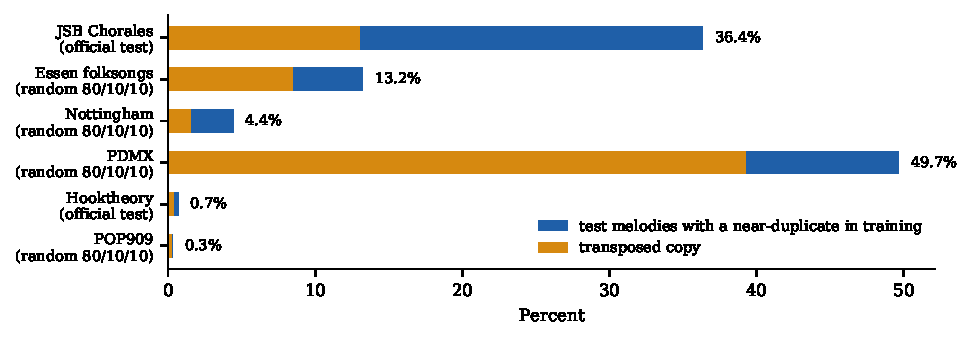
\includegraphics[width=0.95\textwidth]{figures/fig1_audit.pdf}
\caption{Share of test melodies with a near-duplicate (blue) or transposed copy (orange) in the training split, for the official split where one exists and a random 80/10/10 split otherwise.}
\label{fig:audit}
\end{figure*}
% ------------------------------------------------------------

Table~\ref{tab:audit} and Figure~\ref{fig:audit} give the results. The leaks follow the way each corpus was assembled.

\paragraph{JSB Chorales.} Of the 77 official test chorales, 28 (36.4\%) have a soprano twin in the 229 training chorales and 10 (13.0\%) have a transposed copy. Counting a longest common run of half the shorter soprano, 33 (42.9\%) are leaked; the validation split is similar (26.3\% twins, 10.5\% copies). The same comparison on all four voices finds no test chorale with a polyphonic twin. The reason is musical: Bach set the same chorale melodies several times, with different harmonizations, and the random split separated the settings. Figure~\ref{fig:jsbpair} shows one pair; the two pieces have the same soprano and agree in all four voices on 63\% of their frames. Because the benchmark transposes every chorale to a common key, most twins appear in the same key, so even a pitch-level model sees them as identical lines. The official split leaks as much as a random split would (38.5\% on average), which is what a split made without regard to hymn tunes should produce. Matching the sopranos against the music21 Bach corpus identifies the hymn tune for many pieces; we use that only to describe the pairs, since the benchmark carries no identifiers.

% ------------------------------------------------------------
\begin{figure}[t]
\centering
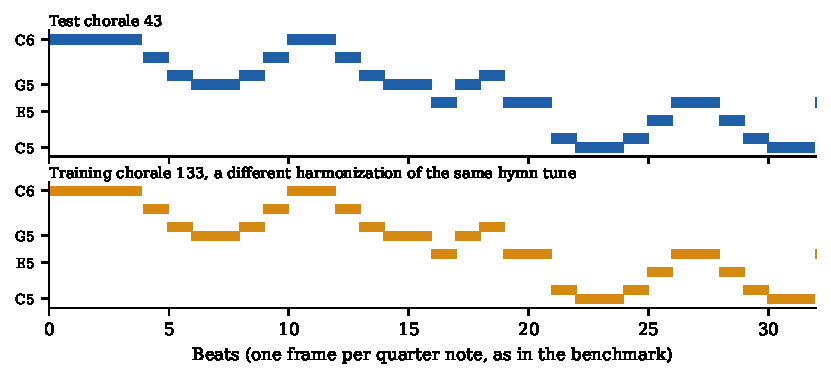
\includegraphics[width=\columnwidth]{figures/fig2_jsb_pair.pdf}
\caption{A transposed twin in the JSB Chorales benchmark: soprano of test chorale 43 and of training chorale 133, first 32 beats. The sopranos are identical; the harmonizations differ on 37\% of frames.}
\label{fig:jsbpair}
\end{figure}
% ------------------------------------------------------------

\paragraph{PDMX.} More than half of the PDMX melodies have a near-duplicate and 39.2\% have a transposed copy, typically the same piece uploaded by several users, a part extracted from an arrangement, or an exercise copied between method books. A random split would give half of all test melodies a twin in training. PDMX ships a deduplicated subset built from metadata embeddings and note counts \citep{long2025pdmx}. Inside that subset 15.2\% of melodies still have a twin and 6.2\% a transposed copy, mostly scores whose titles differ (translations, catalogue numbers, arrangement credits).

\paragraph{Folk and popular corpora.} Essen contains the expected tune families: 16.1\% of its songs have a twin and a random split leaks 13.2\% of test songs. Nottingham's official split leaks 2.4\% and a random split 4.4\%. Hooktheory shows that a split designed against leakage works: its artist-stratified test split leaks 0.7\% of melodies, a quarter of the 2.8\% that a random split would leak, and the remaining twins are covers and misspelled artist names. POP909 has two pairs.

%%%%%%%%%%%%%%%%%%%%%%%%%%%%%%%%%%%%%%%%%%%%%%%%%%%%%%%%%%%%%%%%%%%%%%%%%%%%%%%%
\section{What a leak is worth}\label{sec:counterfactual}

A leaked test piece will usually score better than a clean one, but leaked pieces may also be easier for other reasons. Comparing leaked and clean test pieces within one model therefore does not measure the effect of the leak. We use retraining instead.

\subsection{Design}
For each model we train two arms on JSB Chorales. Arm A uses the official training split. Arm B uses the same split minus the 25 training chorales that twin one of the 28 leaked test chorales (229 chorales become 204). The validation split, the hyperparameters and the random seeds are the same in both arms, so the only difference is the presence of the twins. For each test piece $i$ we record the change in negative log-likelihood $\Delta_i = \mathrm{NLL}_i^{B} - \mathrm{NLL}_i^{A}$. Removing 25 chorales also removes ordinary training data, which hurts every test piece a little; the clean test pieces measure that. The leak benefit is the difference in differences \citep{angrist2009mostly}
\begin{align}\label{eq:did}
\hat{\tau} = \frac{1}{|\mathcal{L}|}\sum_{i \in \mathcal{L}} \Delta_i - \frac{1}{|\mathcal{C}|}\sum_{i \in \mathcal{C}} \Delta_i,
\end{align}
with $\mathcal{L}$ the 28 leaked and $\mathcal{C}$ the 49 clean test chorales. We report the mean over three seeds and a 95\% interval from a bootstrap over test pieces of the seed-averaged $\Delta_i$.

\subsection{Models}
\textit{Soprano models.} The soprano line of each chorale becomes a token sequence of alternating pitch and duration tokens (61 pitches from C2 to C7, a rest, and 17 durations from a twelfth of a beat to eight beats). We train a 4-gram model over note tokens with interpolated absolute-discount backoff in the style of \cite{kneser1995improved}, and decoder-only transformers \citep{vaswani2017attention} with rotary position embeddings \citep{su2024roformer} at three sizes: 0.46M parameters (width 96, four layers), 1.8M (width 192, four layers) and 7.4M (width 320, six layers). Transformers see 1.5M tokens with AdamW, a cosine schedule, dropout 0.1 and a random transposition of $-5$ to $+6$ semitones per epoch, the usual augmentation for melody models. NLL is reported in nats per note, the sum over the pitch and duration tokens.

\textit{Polyphonic models.} To connect with the published benchmark numbers we also train frame-level transformers on the full piano rolls, predicting the 88 binary keys of each frame from the previous frames, at 0.11M and 1.26M parameters with early stopping on the validation split. NLL is reported in nats per frame, the unit used in the JSB literature \citep{boulangerlewandowski2012,bai2018tcn}.

\subsection{Results}

% ------------------------------------------------------------
\begin{table}[t]
\centering
\small
\begin{tabular}{lrrr}
\toprule
\colhead{Model} & \colhead{Leak benefit $\hat\tau$} & \colhead{95\% CI} & \colhead{Seeds} \\
\midrule
\multicolumn{4}{l}{\textit{Soprano, nats per note}} \\
4-gram & \textbf{0.555} & [0.333, 0.784] & 1 \\
Transformer 0.46M & 0.011 & [0.001, 0.020] & 3 \\
Transformer 1.8M & 0.026 & [0.012, 0.042] & 3 \\
Transformer 7.4M & 0.060 & [0.039, 0.080] & 3 \\
\midrule
\multicolumn{4}{l}{\textit{Four voices, nats per frame}} \\
Transformer 0.11M & 0.055 & sd 0.005 & 3 \\
Transformer 1.26M & 0.249 & sd 0.059 & 3 \\
\bottomrule
\end{tabular}
\caption{What the JSB leak is worth: the difference in differences of Equation~\ref{eq:did} after retraining without the 25 training twins. The 4-gram is deterministic, so its interval reflects only the choice of test pieces. For the four-voice models we report the standard deviation over seeds.}
\label{tab:did}
\end{table}
% ------------------------------------------------------------

% ------------------------------------------------------------
\begin{figure*}[t]
\centering
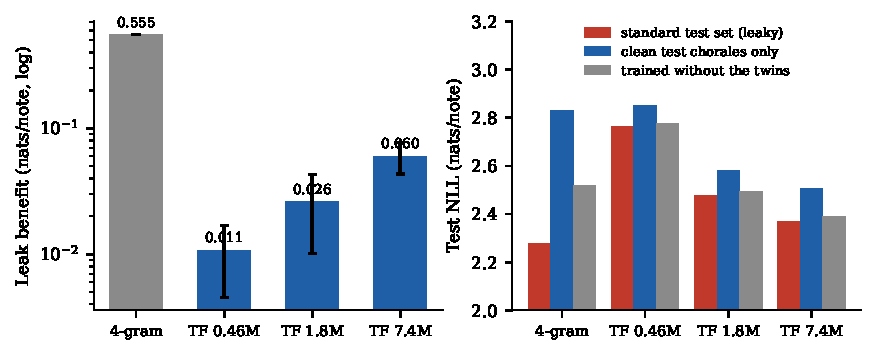
\includegraphics[width=0.95\textwidth]{figures/fig3_counterfactual.pdf}
\caption{Left: leak benefit by model (log scale; error bars are one standard deviation over seeds). Right: NLL on the official test set, on its clean chorales only, and on the official test set after retraining without the twins. On the official test set the 4-gram looks best; on clean pieces the two larger transformers beat it.}
\label{fig:counterfactual}
\end{figure*}
% ------------------------------------------------------------

Table~\ref{tab:did} and Figure~\ref{fig:counterfactual} give the results.

\paragraph{The leak rewards copying.} The 4-gram gains 0.555 nats per note from the twins, and 0.788 on the ten test chorales whose twin is a transposed copy. The transformers gain 0.011 to 0.060 nats per note, with no difference between copies and partial twins. A count model memorizes every phrase it has seen and can only generalize by backing off, so a test piece whose phrases are all in the training data is the best case for it. The transposition augmentation used for the transformers works against exact recall of the leaked pitch strings.

\paragraph{The leak reverses a ranking.} On the official test set the 4-gram scores 2.278 nats per note, better than every transformer (the best scores 2.371). On the 49 clean test chorales the 4-gram scores 2.832, the two larger transformers beat it by 0.25 and 0.33 nats per note, and the smallest ties it (2.850). A reader of the official numbers would rank the count model first. Retraining confirms that the leak causes the reversal: with the twins removed from training, the 4-gram falls from 2.278 to 2.517 on the official test set and drops behind the two larger transformers, whose scores move by 0.02 nats or less.

\paragraph{The benefit grows with capacity.} Among transformers the leak benefit rises from 0.011 to 0.026 to 0.060 nats per note as parameters grow sixteenfold, and the intervals for the smallest and largest model do not overlap. The four-voice models show the same pattern: the leak is worth 0.055 nats per frame at 0.11M parameters and 0.249 at 1.26M, a 4.5-fold increase for an elevenfold increase in size (Table~\ref{tab:did}). Larger models are the ones papers report as improvements, so a leaked benchmark inflates exactly the comparisons it is used for. Published four-voice results on JSB differ from each other by amounts of the same order: \cite{bai2018tcn} report 8.10 nats per frame for a temporal convolutional network against 8.45 for an LSTM.

%%%%%%%%%%%%%%%%%%%%%%%%%%%%%%%%%%%%%%%%%%%%%%%%%%%%%%%%%%%%%%%%%%%%%%%%%%%%%%%%
\section{Memorization at melody-model scale}\label{sec:memorization}

The counterfactual measures how much a model gains from having seen a twin. A related question is whether melody models reproduce their training melodies verbatim, as language models reproduce text \citep{carlini2021extracting}. We study this on PDMX, which is public domain or CC0 and so can be released together with any extracted melodies.

\subsection{Design}
We split PDMX by twin family rather than by melody: 3\% of the families are held out whole for testing, so no test melody has a twin in training, and 15\% of the remaining families form the training pool. The \textit{raw} corpus keeps every melody in the training families (29,208 melodies, natural duplication intact); the \textit{dedup} corpus keeps one melody per family (18,089). Both corpora receive the same 360 canaries: synthetic melodies of 48 notes, built as scale-constrained random walks over common rhythm cells, inserted 1, 2, 4, 8, 16 or 32 times (60 canaries per level). Another 60 canaries are generated the same way and never inserted. Each model is trained on 30M tokens, which is 3.0 passes over the raw corpus and 4.8 over the dedup corpus, so a canary inserted 32 times is seen about 100 to 150 times. Training uses the same transposition augmentation as above unless stated. To look for the onset of memorization we also train the 1.8M model on a pool one fifth the size (5,887 melodies, 13 passes), with and without augmentation.

We measure three things. \textit{Canary extraction}: prompted with a canary's first 12 notes, does greedy decoding reproduce the next 20 notes exactly? \textit{Canary exposure}: the NLL of inserted canaries against never-inserted ones. \textit{Natural extraction and copying}: the same extraction test on real training melodies grouped by family size, and, for 300 unconditional samples at temperatures 0.8 and 1.0, the longest passage that matches one training melody contiguously up to transposition and tempo. Because repeated notes, trills and scale runs occur in thousands of scores, we also report the longest \textit{non-trivial} shared passage, one with at least four distinct intervals, at most half repeated notes, and no cell of up to eight notes looped through it.

\subsection{Results}
Table~\ref{tab:mem} gives the results.

\begin{table*}[t]
\centering
\small
\begin{tabular}{lrrrrrrr}
\toprule
\colhead{Run} & \colhead{Test NLL} & \colhead{Exposure $\times$1} & \colhead{Exposure $\times$32} & \colhead{Extract $\times$32} & \colhead{Natural extract} & \colhead{Any run $\geq$20} & \colhead{Longest non-trivial} \\
\midrule
0.46M raw & 2.636 & -0.083 & +0.025 & 0\% & 0.0\% & 1\% & 15 \\
1.8M dedup & 1.877 & -0.064 & +0.023 & 0\% & 0.0\% & 8\% & 19 \\
1.8M raw & 1.777 & -0.076 & +0.031 & 0\% & 0.0\% & 22\% & 19 \\
\bottomrule
\end{tabular}
\caption{Memorization on PDMX. \textit{Exposure}: NLL of 60 never-inserted canaries minus NLL of 60 canaries inserted 1, 8 or 32 times, in nats per note (positive means the model prefers the inserted canaries). \textit{Extract}: share of canaries inserted 32 times whose next 20 notes greedy decoding reproduces exactly from a 12-note prompt. \textit{Natural extract}: the highest extraction rate over real training melodies grouped by family size. \textit{Any run}: share of 300 unconditional samples at temperature 0.8 that share a contiguous passage of at least 20 notes with one training melody, up to transposition. \textit{Longest non-trivial}: the longest such passage, in notes, among passages with at least four distinct intervals and at most half repeated notes. Test NLL is on held-out families and is comparable only between runs with the same training pool.}
\label{tab:mem}
\end{table*}


\paragraph{No verbatim recall.} No model reproduces any canary from its 12-note prompt, including the canaries inserted 32 times and seen about a hundred times during training. No model reproduces any real training melody either, including members of families with ten or more copies in the raw corpus. Canary exposure stays within 0.1 nats per note of zero at every insertion level. The canaries inserted 32 times are slightly preferred (by 0.02 to 0.03 nats per note), an effect smaller than the spread between the lower insertion levels.

\paragraph{Copying in free samples is generic.} Long shared passages do appear in free samples: 22\% of samples from the 1.8M model trained on the raw corpus share a contiguous run of at least 20 notes with some training melody, against 8\% for the same model trained on the deduplicated corpus. Every one of these runs is a repeated note, a trill or a two-note figure. Among non-trivial passages, the longest that any sample shares with any training melody is 19 notes. Deduplication therefore changes what the model produces, cutting the share of samples dominated by figuration, without any sign that the raw model was reproducing tunes.

\paragraph{Reading the two studies together.} At the scale typical of symbolic melody models, transformers trained with transposition augmentation do not store their training melodies in a retrievable form, yet they still score leaked test melodies better than clean ones by an amount that grows with capacity (Section~\ref{sec:counterfactual}). A leak can therefore inflate a benchmark without any detectable memorization, and checking for verbatim copies is no substitute for checking the split.


%%%%%%%%%%%%%%%%%%%%%%%%%%%%%%%%%%%%%%%%%%%%%%%%%%%%%%%%%%%%%%%%%%%%%%%%%%%%%%%%
\section{Released resources and recommendations}\label{sec:release}

We release, under the MIT licence for code and CC0 for derived data where the source permits:
\begin{itemize}
\item the twin detector and the audit pipeline, with tests;
\item twin lists for JSB Chorales, Nottingham, Hooktheory, POP909 and PDMX, each pair with its Jaccard score, longest common run and transposition;
\item a leakage-free JSB evaluation set (the 49 clean test chorales) and a family-level re-split of all 382 chorales, and family-level splits of PDMX and Nottingham;
\item the trained memorization models and their canaries;
\item an interactive page where JSB and PDMX twins can be played side by side.\endnote{\url{https://takakhoo.com/melodies}}
\end{itemize}
Essen twin lists are given as identifier pairs only, because the collection's terms do not allow redistribution of the melodies.

For authors evaluating melody models we suggest three practices. First, split by tune family, using a transposition-invariant detector to build the families, or report results on a clean subset of the test set alongside the standard number. Second, when a corpus is assembled from many uploaders, as PDMX is, deduplicate at the melody level and keep the family structure for splitting. Third, include a copy-prone baseline such as an $n$-gram or PPM model \citep{pearce2005thesis}; if it does unexpectedly well on a test set, look for leaks.

%%%%%%%%%%%%%%%%%%%%%%%%%%%%%%%%%%%%%%%%%%%%%%%%%%%%%%%%%%%%%%%%%%%%%%%%%%%%%%%%
\section{Limitations}\label{sec:limits}

The detector measures melodic identity. Two melodies can share half their phrases and still be distinct compositions, as with tunes built from stock formulas; a twin can also be a deliberate variant that a musicologist would want in both sets. Our thresholds favour precision, so the reported leak rates are lower bounds for near-duplicates in a broader sense. The counterfactual uses one benchmark with 28 leaked pieces; the intervals are correspondingly wide, and the transformers we train are small by current standards. The memorization study covers models up to 7.4M parameters and at most 13 passes over the data; larger models trained for longer may well memorize. Our extraction test is strict (20 exact notes from a 12-note prompt), and the copy search only finds contiguous passages. We do not analyse The Session or IrishMAN, two of the corpora most likely to contain tune families, because of their licence terms.

%%%%%%%%%%%%%%%%%%%%%%%%%%%%%%%%%%%%%%%%%%%%%%%%%%%%%%%%%%%%%%%%%%%%%%%%%%%%%%%%
\section{Conclusion}\label{sec:conclusion}

Melodies travel in versions, and the standard splits of melody corpora were drawn without that in mind. In JSB Chorales more than a third of the test set repeats a training soprano. In PDMX half of a random test set would. Retraining without the twins shows that the leak is worth an order of magnitude more to a copy-prone model than to a transformer, enough to reverse a ranking, and that among transformers the benefit grows with size, even though the transformers show no verbatim memorization. A transposition-invariant audit costs minutes on a laptop. We hope the released tools make it a routine step before a melody benchmark number is reported.

%%%%%%%%%%%%%%%%%%%%%%%%%%%%%%%%%%%%%%%%%%%%%%%%%%%%%%%%%%%%%%%%%%%%%%%%%%%%%%%%
\section{Reproducibility}
All code, configuration files and result files are available in the project repository.\endnote{\url{https://github.com/takakhoo/transformer-melody-generation}} Every number in this article is produced by a numbered experiment script from the downloaded corpora, and every experiment runs on a laptop CPU.

\section{Ethics and consent}
All corpora are used under their published terms. PDMX scores are public domain or CC0. Essen melodies are counted but never redistributed. The Session and IrishMAN are excluded because The Session's licence forbids processing with language-model tools. No human participants were involved.

\nolinenumbers
\theendnotes

\section*{Competing Interests}
The author has no competing interests to declare.

\section*{Authors' Contributions}
TK designed the study, wrote the code, ran the experiments and wrote the article.

\begin{authoraff}[AUTHOR AFFILIATIONS]
\end{authoraff}
\clearpage

\bibliographystyle{apaTISMIR}
\bibliography{references}

\label{endPage_Label}
\end{document}
